\begin{tikzex-nobt}{11.45}
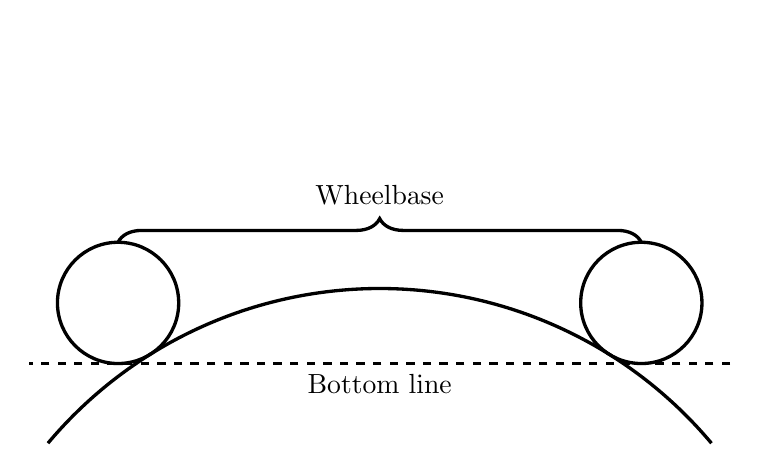
\begin{tikzpicture}[very thick,scale=0.55]
  \draw (40:10cm) arc (40:140:10cm);
  \draw (58:11.4cm) circle[radius=1.4cm]
       (122:11.4cm) circle[radius=1.4cm];

  \draw (58:11.4) ++(0,-1.4) coordinate(a);
  \draw (122:11.4) ++(0,-1.4) coordinate(b);

  \draw[dashed] (36:10cm |- a) -- (144:10cm |- b)
       node[midway,below]{Bottom line};

  \draw[decorate,decoration={brace,mirror,
       amplitude=3mm,raise=15.4mm}] (a) -- (b)
       node[midway,above,
            inner sep=20mm]{Wheelbase};
\end{tikzpicture}
\end{tikzex-nobt}
